\chapter{VIRTUAL BACKBONE DETERMINATION IN WIRELESS SENSOR NETWORKS} \label{ch:WSN}% Must have a blank line after every section label

\section{Background} \label{sec:background} % Must have a blank line after every section label

Sensor networks have a long history. The first obvious sensor network wa the \ac{SOSUS} which grew out of tasking in 1949\cite{whitman2005sosus,chong2003sensor}. The \ac{SOSUS} was made up of acoustic sensors that were interconnected by wired cables and were deployed by the US in deep ocean basins during the Cold War to detect and track Soviet submarines. The early development of sensor networks was mainly driven by military use, in which sensor nodes were wired together to provide battlefield surveillance. Advances in \ac{MEMS} technology, wireless communications, and digital electronics have enabled the development of low-cost, low-power, multifunctional sensor nodes that communicate untethered in short distances\cite{akyildiz2002wireless}. Such sensors can observe and respond to phenomena in the physical environment and they have driven sensor networks to the \acp{WSN}.

The \ac{WSN} can be defined as a self-configured and infrastructure-less network composed of autonomous resource-limited electronic sensors geographically distributed across a region where the sensors communicate with each other wirelessly\cite{carlos2016wireless,saibharath2014virtual}. \acp{WSN} have been the focus of intense research during the past few years because of their potential to facilitate data acquisition and scientific studies\cite{werner2006deploying}. These inexpensive small miniaturized sensors can be embedded or scattered onto target environments in order to observe or monitor useful information in many situations. Wireless communication between sensors allows the formation of flexible sensor networks, which can be deployed rapidly over wide or inaccessible areas. Thus, \acp{WSN} greatly extend our ability to monitor and control the physical environment. Some of the main applications are habitat and ecosystem monitoring, seismic monitoring, civil structural health monitoring, volcano monitoring, groundwater contamination monitoring, outer space investigations and so on\cite{senniappan2016application,werner2006deploying,prasad2011wireless,hong2002load,xue2010two}.  The communication in \acp{WSN} can be either ad hoc (multi-hop) or single-hop wireless transmission\cite{akyildiz2002wireless,meghji2011transmission,singh2015design}. Although the latter is popular in short-range applications, such as home control and building automation, the former, ad hoc technique will be the focus of the engineering project of this chapter due to its high flexibility and ability to support long-range, large-scale, and highly distributed applications\cite{singh2015design}.

\section{Problem Specification} \label{sec:problem}

In a \ac{WSN}, after collecting information from the environment, sensors need to transmit aggregated data to sink nodes (gateways) or information collection nodes. Due to the small scale and limited communication capability of sensors, a packet sent from one sensor to another usually has to go through multiple hops, which makes routing a critical service required for \acp{WSN}. For sustenance of the network, one must have both energy efficient transmission and high overall network lifetime. The main goal is to minimize the energy consumed and maximize the network lifetime. Clustering and backbone formation are two contrasting schemes for efficient routing in wireless sensor network\cite{tandon2012determination}. Basically every node will transfer its message to its cluster head and the cluster head would communicate to sink via many intermediate cluster head.

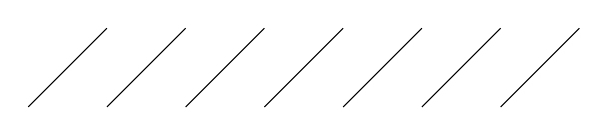
\begin{tikzpicture}
     \foreach \x in {1,2,3,4,5,6,7}{%
       \pgfmathadd{\x}{1}
       \pgfmathsetmacro{\y}{\pgfmathresult};
       \draw (\x,0) -- (\y,1);
     }
   \end{tikzpicture}